\documentclass[UTF8]{ctexart}

\usepackage{subfiles}  

%下面的语句, 引入你的头部设置文件
\usepackage{C:/phpStorm_proj/02_myself_ID_EGO/+100_latex_all_math_sel/myPreamble} 
%必须是绝对路径,才能让各个tex在单独编译时使用到

\title{文件名}


%---------------------------------


\begin{document}
	\tableofcontents % 生成目录
	\date{} % 若不写这句, 则默认也会渲染出日期, 所以我们要手动赋空值
	\maketitle  %这行代码, 让你前面的 title, author, date生效

	\part{正态分布 and 标准正态分布}
	
	\section{正态分布, normal distribution}
	
	正态分布, normal distribution, 直译过来就是``最常态下的分布", ``一般最常见的分布". 它又名高斯分布 Gaussian distribution.  \\
	正态分布, 是概率分布中最重要的分布. 在数学家眼里,它是远远高于其他分布的. 有很多其他的分布,比如对数正态分布、T分布、F分布, 都是直接由``正态分布"推导出来的. \\
	
	
	
	
	
	
	
	
	
	
	

\subsection{正态分布 - 概率密度函数 : $\boxed{
	\varphi (x)=\frac{1}{\sqrt[]{2\pi}\cdot \sigma}e^{-\frac{(x-\mu )^2}{2\sigma ^2}}
}$ }

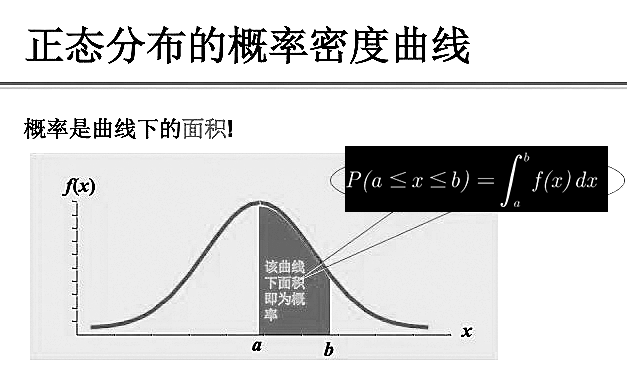
\includegraphics[width=0.7\textwidth]{/0212.png} \\

	
	概率密度函数. 用小写的 $\varphi$ 表示. \\
	``正态分布" $N(\underset{\text{平均值}.}{\underbrace{\mu }},\underset{\sigma \text{是标准差.\ }\sigma ^2\text{是方差}}{\underbrace{\sigma ^2}})	$ 的概率函数是: 
	 $\boxed{
		\varphi (x)=\frac{1}{\sqrt[]{2\pi}\cdot \sigma}e^{-\frac{(x-\mu )^2}{2\sigma ^2}} \ (-\infty <x<+\infty )
	}$  \\
\vspace{1em} 

	记作: $\boxed{X \sim N(\mu ,\sigma ^2)}$   ← 称为: X服从``参数为$\mu$, $\sigma$的正态分布(或高斯分布)". \\	
	- 这里的 N, 就是正态分布 (Normal distribution) 的英文首字母.\\
	- $\mu$ 是 ``平均值" \\
	- $\sigma$ 是 ``标准差" \\
	- 注意: 概率函数公式里, 这第二个参数写的是$\sigma ^2$, 而不是$\sigma$! 所以, 比如对于N(1, 100)来说, 其 $\mu=1$,  $\sigma ^2=100$, 即$\sigma=10$. \\
	- 在正态分布中,``平均值 $\mu$"等于``期望",它决定了这条曲线的最高点; ``方差$\sigma^2$"决定胖瘦,它决定曲线的弯曲度. 简单这两个数据,就确定了这条曲线的形状. \\
	
	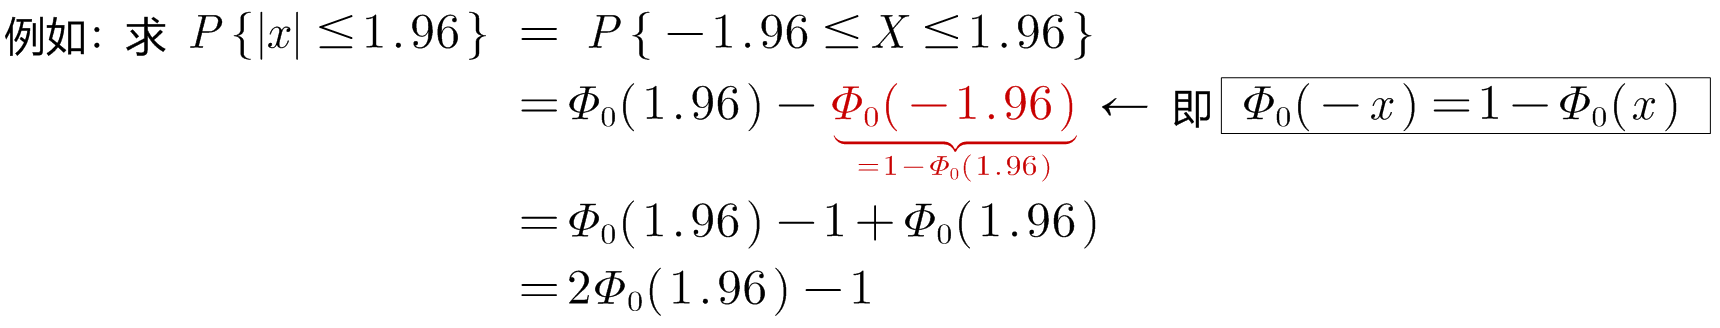
\includegraphics[width=0.4\textwidth]{/0186.png} \\
	
	
	正态分布的 f(x)曲线 : \\
	- 横坐标, 代表随机变量X的取值范围. 越往右, 随机变量的值就越大. \\
	- 纵坐标, 则代表概率的大小,最底下的概率是0, 越往上概率越大. \\	
	这样,从曲线上随便找一点,确定它的横坐标、纵坐标,我们就知道了这个值出现的概率是多少. \\
	
	因为这条曲线是左右对称的,所以 : \\
	- 中间的最高点,就代表\textbf{``平均值"出现的概率最大,数据最多.} \\
	- 而两边陡峭下降,就意味着: \textbf{越靠近平均值,数据越多; 越远离平均值,数据就越少.} 
	


	
	
	
	\subsection{正态分布 - 累加函数 : $\boxed{
			F(x)=\frac{1}{\sqrt[]{2\pi}\cdot \sigma}\int_{-\infty}^x{\left[ e^{-\frac{(x-\mu )^2}{2\sigma ^2}} \right]}dx
		}$ }
	
	对``概率函数 f(x)"求积分, 其曲线下的阴影面积就是``累加函数 F(x)". 其面积=1. \\
	
	
	\begin{align*}  % 支持每行编号. 若不需要编号, 就用 align*环境
	&\underset{\text{累加函数}}{\underbrace{F(x)}}=\int_{}^{}{\underset{\text{概率函数}}{\underbrace{f(x)}}}dx\\
&=\int_{-\infty}^x{\left[ \frac{1}{\sqrt[]{2\pi}\cdot \sigma}e^{-\frac{(x-\mu )^2}{2\sigma ^2}} \right]}dx\\
&=\frac{1}{\sqrt[]{2\pi}\cdot \sigma}\int_{-\infty}^x{\left[ e^{-\frac{(x-\mu )^2}{2\sigma ^2}} \right]}dx
	\end{align*}



\vspace{1em} 
\subsection{正态分布(钟形曲线)的``概率函数"的性质}



\subsubsection{以 ``x=均值$\mu$" 为对称轴}

正态分布的``概率函数"曲线, 以 ``x=均值$\mu$" 为对称轴. 在此处, 函数的y值达到最大. 即此时 $y=\dfrac{1}{\sqrt[]{2\pi}\cdot \sigma}$ \\

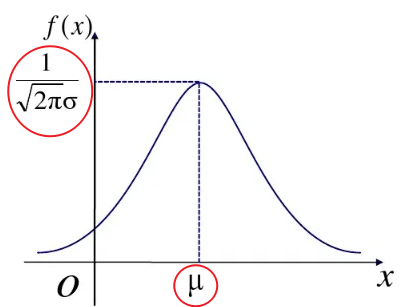
\includegraphics[width=0.35\textwidth]{/0187.png} \\

所以, 对称轴$\mu$, 能控制图像的``左右平移". \\

\textbf{均值就是期望.} 它们重合在同一点处 --- 即``曲线中间的最高点"的x坐标处. \\
\textbf{数学期望, 代表``长期中的价值为几许?". 在正态分布中,``平均值"就能代表随机事件的长期价值.} \\

为什么我们会用高考的平均成绩,衡量一所高中的教学质量? 为什么我们会用平均收益率,衡量一家基金公司的好坏? 原因很简单,因为高考成绩和基金公司的收益,都是服从``正态分布"的.




\subsubsection{极端值很少. 且``极端值"对``均值"的影响很小}
正态分布的图形, 越靠近平均值,这条曲线越高,出现的概率越大; 越远离平均值,这条曲线就越低,出现的概率就越小. 这就说明,\textbf{正态分布的大多数数据, 都集中在平均值附近,极端值很少.} \\

``极端值很少"这句话,有两层含义:  \\
- 一是\textbf{极端值出现的概率很低} \\
- 二是\textbf{极端值对``均值"的影响很小} \\

也因此,正态分布中的数据是非常稳定的. 比如人的身高,它大体服从正态分布,\textbf{所以即使姚明加入我们课程, 我们的平均身高也不会有太大变化 (即: ``极端值"对``均值"的影响很小).}




\subsubsection{以x轴为渐近线}
就是说, 曲线的两端, 无限接近于 y=0, 而不会掉落到 -y 领域上去.



\subsubsection{在 $x=\mu \pm \sigma $ 处有``拐点"}
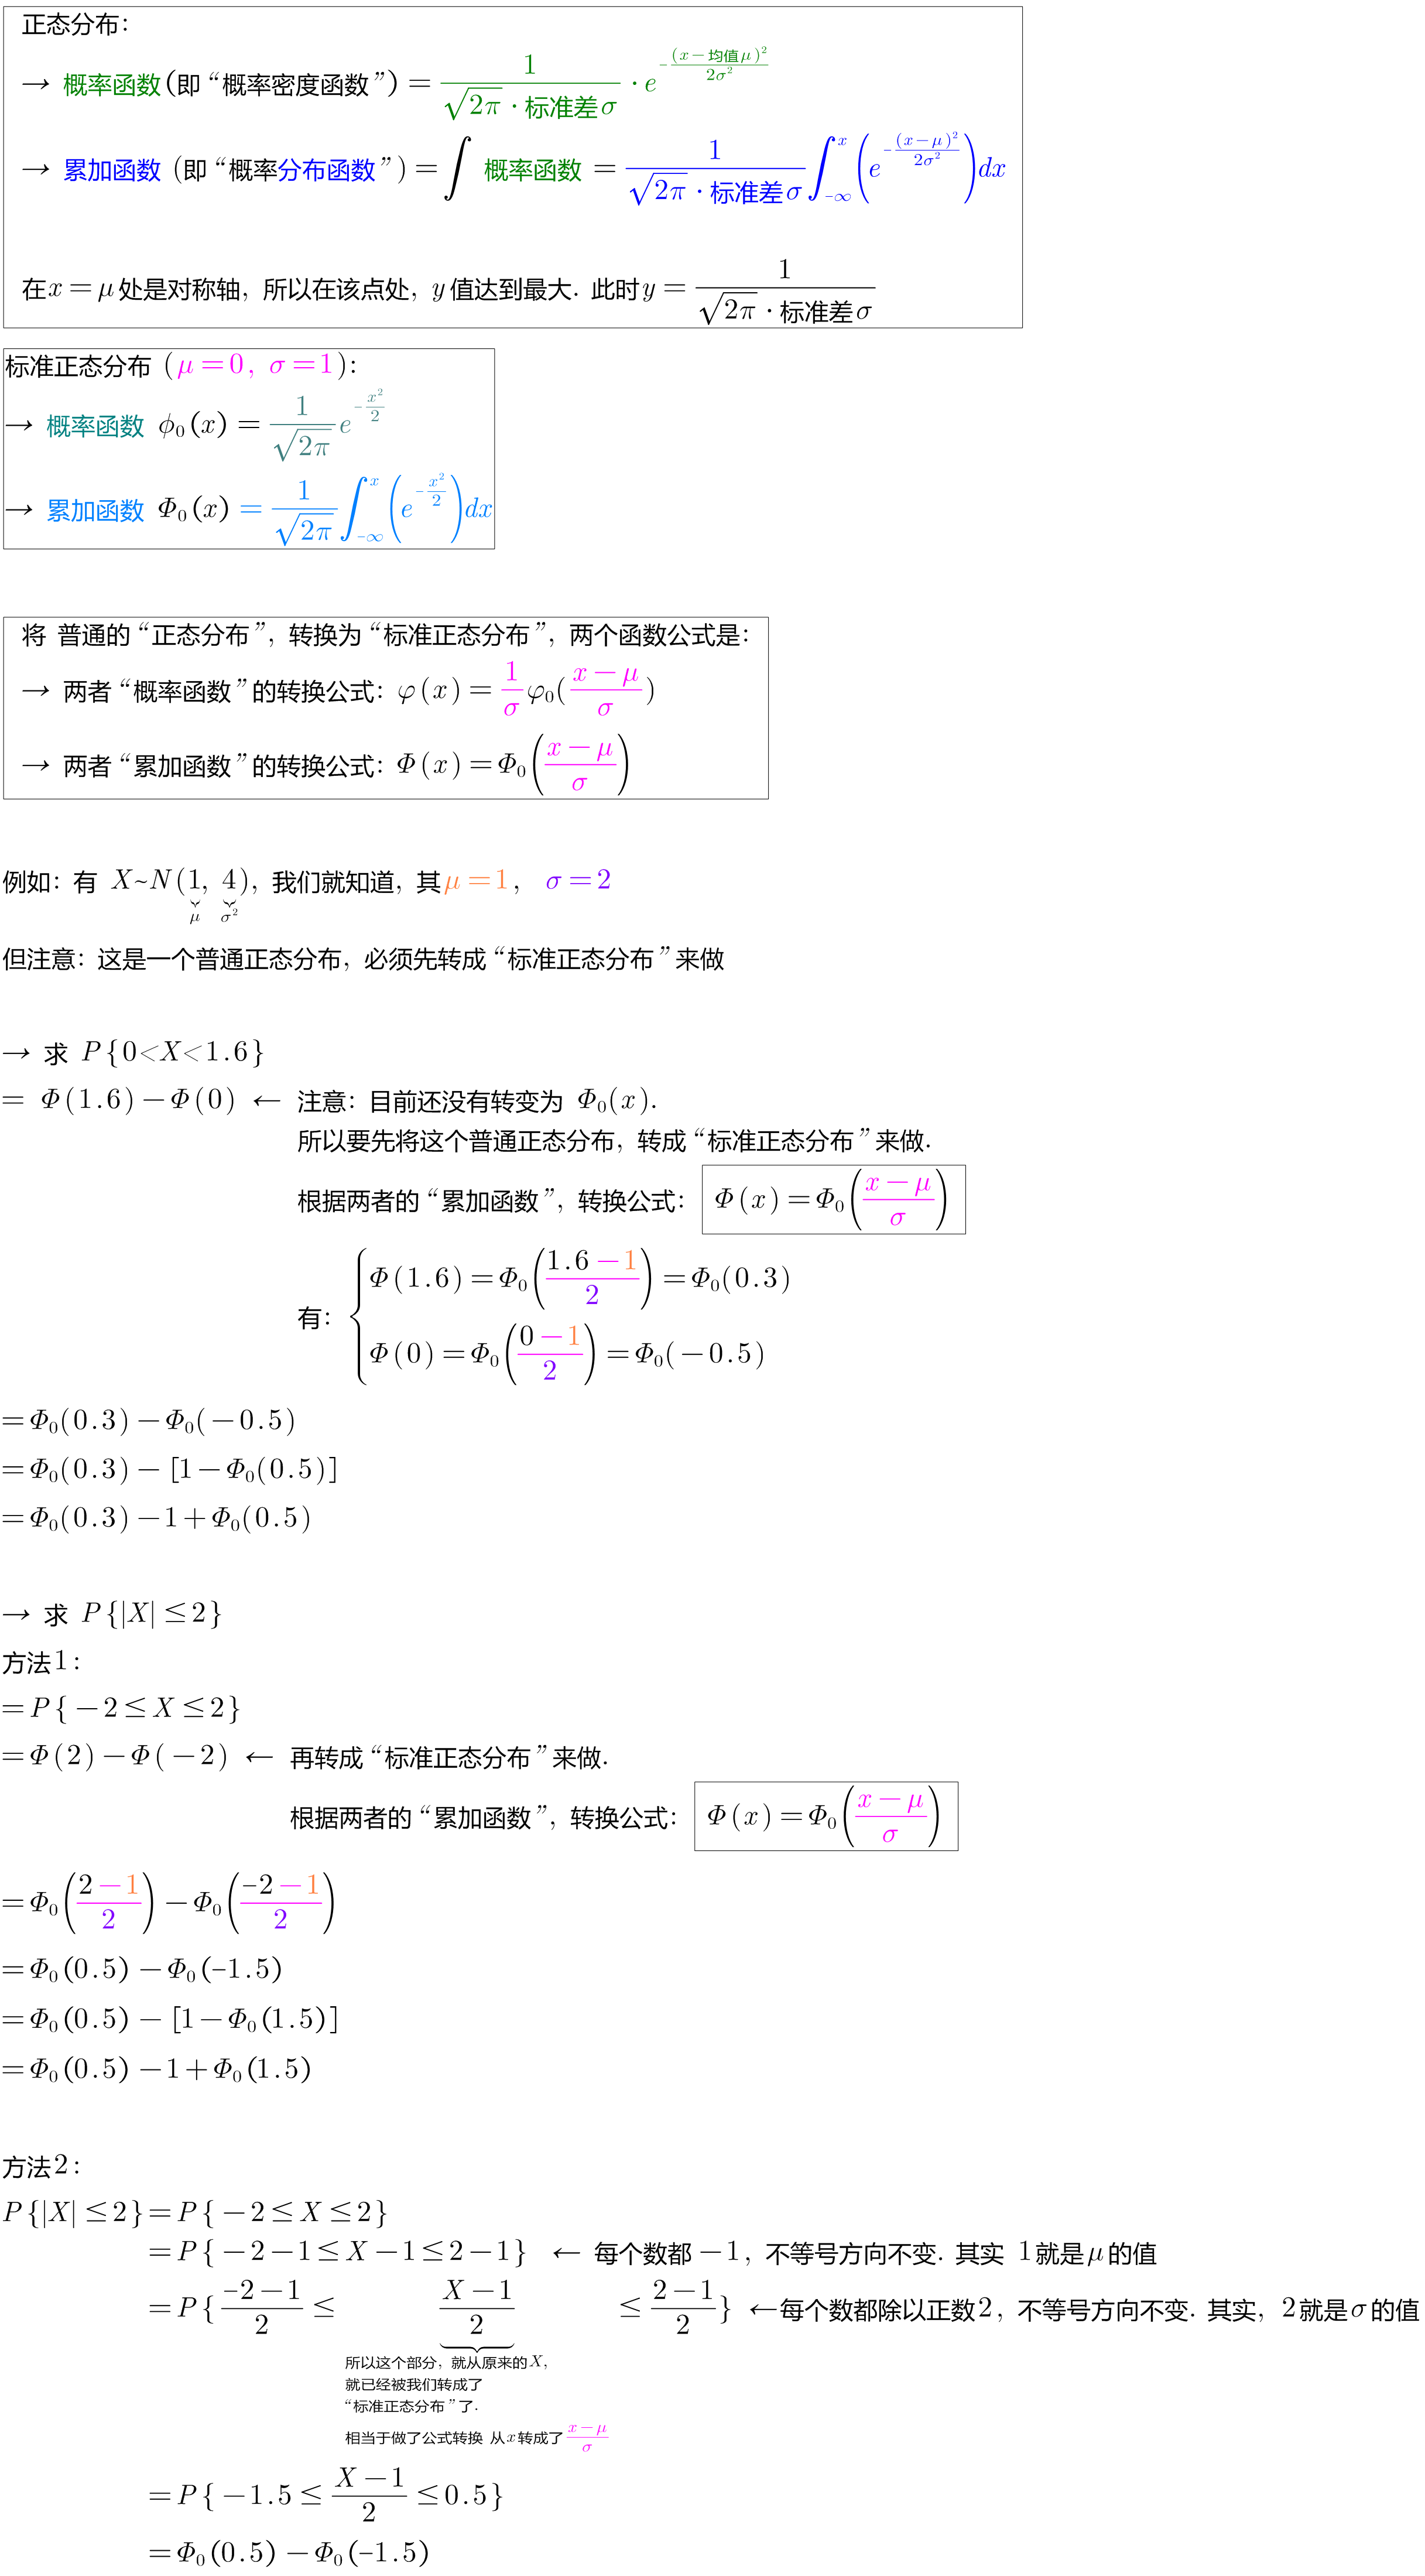
\includegraphics[width=0.7\textwidth]{/0188.png} 



\subsubsection{``$\sigma$ 标准差"参数, 控制图像的``矮胖"或``高瘦"}

→ 若$\sigma$ 变小: 因为 在x=μ处, y有最大值是 $ \dfrac{1} {\sqrt{2π} \cdot \sigma}$. 所以 当$\sigma$ 变小时, 分母变小, 则分数值就变大, 即y值变大, 所以图像会拉高, 变瘦高. \\
→ 若$\sigma$ 变大: 则最高点的y值变小, 图像会压低, 变矮胖. \\

- 标准差$\sigma$越大,数据的波动越剧烈,钟形曲线就越矮胖 (即x轴的横跨幅度越大). \\
- 标准差$\sigma$越小,波动就越小, 数据就越集中,钟形曲线就越高瘦 (即x轴的横跨幅度越窄). \\


但注意, 无论是变瘦高, 还是变矮胖, 曲线下的阴影面积, 始终是=1, 不变的! \\

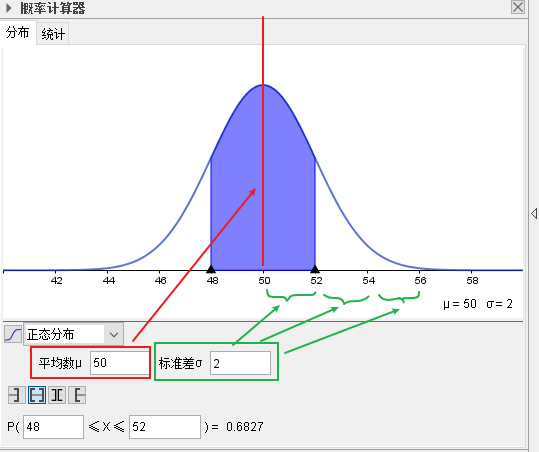
\includegraphics[width=0.65\textwidth]{/0189.png} 




\subsubsection{对不同的``正态分布"曲线, 进行比较}

不同的正态分布曲线, 也能进行比较: \\

(1) \textbf{标准差$\sigma$相同, 均值$\mu$不同, 能比较``好坏(即价值高低)".} \\
因为均值即"期望", 期望就代表"长期价值". 两个事物的``期望"不同, 自然它们的价值高低也不同. \\




(2) \textbf{均值$\mu$相同, 标准差$\sigma$不同, 能比较``波动"(即风险性).}  

\begin{myEnvSample}
男女智商的正态分布曲线如下, \\
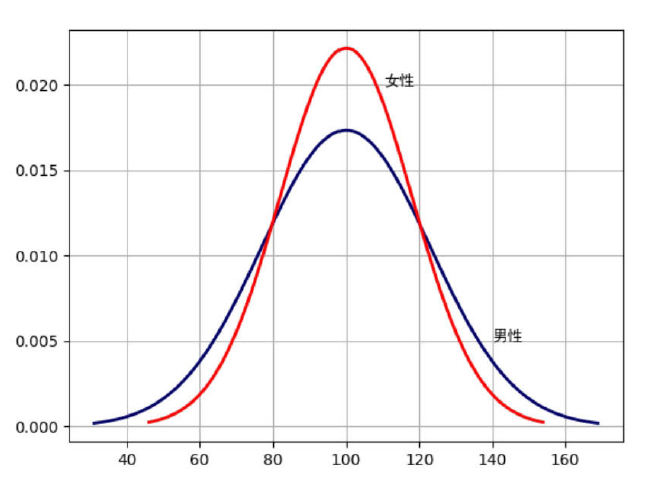
\includegraphics[width=0.6\textwidth]{/0198.png} \\

能看出: \\
- 两者的均值相同. 说明男女智商, 没有高低之分. \\
- 但高矮胖瘦不一样(即"标准差$\sigma$"不一样, 波动程度不一样) : \\
→ 男性智商的波动性更大(即x跨幅更宽, 更矮胖), 说明在智商高的人中间,男性的数量要多于女性 (比如, \textbf{我们看 X=140 智商处, 男性的蓝色曲线的高度, 要高于女性的红色曲线, 说明在 X=140智商处, 男的概率, 要多于女的});  \\
→ 当然,\textbf{智商低下的人中间(比如 X=60智商处),男性也同样比女性多.}
\end{myEnvSample}
\vspace{1em} 



(3) \textbf{均值和标准差, 都不同. 那也能比较``专业和业余"} \\
比如, 某体育项目, 你和世界冠军同台比赛, 他比你得分高(期望大), 又成绩稳定(方差小), 所以这两项都比你强, 就说明他比你``专业". \\
所以, \textbf{专业就是``均值$\mu$更高,标准差$\sigma$更小". 而业余则恰恰相反. }


~\\
\hrule
~\\



\section{标准正态分布 ← 即当 均值$\mu=0$, 标准差 $\sigma=1$ 时的``正态分布"}


\subsection{标准正态分布 - 概率函数 : $\boxed{
		\phi _0(x)=f\left( x \right) =\frac{1}{\sqrt[]{2\pi}}e^{-\frac{x^2}{2}}		
	}$}


我们把$\mu=0, \sigma=1$, 代入正态分布的 PDF 和 CDF 函数中, 就得到: \\

``标准正态分布"的``概率函数 PDF" (专门记作$\phi _0(x)$) :\\
$
\phi _0(x)=f\left( x \right) =\dfrac{1}{\sqrt[]{2\pi}\cdot \underset{=1}{\underbrace{\sigma }}}e^{-\frac{(x-\overset{=0}{\overbrace{\mu }})^2}{2\sigma ^2}}
=\dfrac{1}{\sqrt[]{2\pi}\cdot 1}e^{-\frac{(x-0)^2}{2\cdot 1^2}}
=\dfrac{1}{\sqrt[]{2\pi}}e^{-\frac{x^2}{2}}
$ \\

即: 
 $\boxed{
	\phi _0(x)=f\left( x \right) =\frac{1}{\sqrt[]{2\pi}}e^{-\frac{x^2}{2}}		
}$


\vspace{1em} 
\subsection{标准正态分布 - 累加函数 :  $\boxed{
		\varPhi _0(x)=F\left( x \right) =\frac{1}{\sqrt[]{2\pi}}\int_{-\infty}^x{\left[ e^{-\frac{x}{2}} \right]}dx
	}$}
	

``标准正态分布"的``累加函数 CDF" (专门记作$\varPhi _0(x)$) :
\begin{align*}  % 支持每行编号. 若不需要编号, 就用 align*环境
	\varPhi _0(x) &=F\left( x \right)\\
&=\frac{1}{\sqrt[]{2\pi}\cdot \underset{=1}{\underbrace{\sigma }}}\int_{-\infty}^x{\left[ e^{-\frac{(x-\overset{=0}{\overbrace{\mu }})^2}{2\sigma ^2}} \right]}dx\\
&=\frac{1}{\sqrt[]{2\pi}\cdot 1}\int_{-\infty}^x{\left[ e^{-\frac{(x-0)^2}{2\cdot 1^2}} \right]}dx\\
&=\frac{1}{\sqrt[]{2\pi}}\int_{-\infty}^x{\left[ e^{-\frac{x}{2}} \right]}dx  
\end{align*}

即: $\boxed{
	\varPhi _0(x)=F\left( x \right) =\frac{1}{\sqrt[]{2\pi}}\int_{-\infty}^x{\left[ e^{-\frac{x}{2}} \right]}dx
}$





\vspace{1em} 
\subsection{标准正态分布 的性质}

\subsubsection{因为它的 $\mu=0$, 所以它的函数曲线, 关于 x=0 对称, 即y轴是对称轴.}

所以它就是个偶函数.  有: \\
- 概率函数 $ \varphi_0(x) = \varphi_0(-x) $   ← 我们在下标处加个0, 来表示它是``标准"的正态分布函数的 ``概率函数"或``累加函数". \\

- 其``累加函数"有: $\boxed{\varPhi _0(-x)=1-\varPhi _0(x)}$ ← 这个公式很重要! \\
比如 : $\varPhi _0(-4)=1-\varPhi _0(4)$ \\

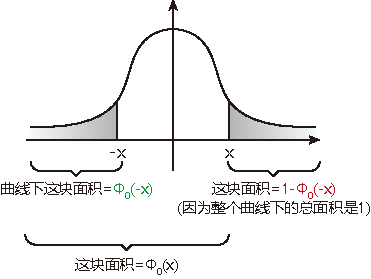
\includegraphics[width=0.5\textwidth]{/0190.pdf} \\
	
	
\begin{myEnvSample}
	\begin{align*}  % 支持每行编号. 若不需要编号, 就用 align*环境
	\text{求} \ P\{|x|\leq 1.96\} &=P\{-1.96\leq X\leq 1.96\}\\
&=\varPhi _0(1.96)-\underset{=1-\varPhi _0(1.96)}{\underbrace{\varPhi _0(-1.96)}}\\
&=\varPhi _0(1.96)-1+\varPhi _0(1.96)\\
&=2\varPhi _0(1.96)-1
	\end{align*}

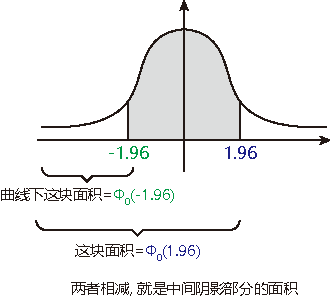
\includegraphics[width=0.5\textwidth]{/0191.pdf} 
\end{myEnvSample}	






\subsubsection{对于 $ x \geq 5$ 的y值, 已经非常靠近y=0了}

正态分布的值, 怎么算? --- 查表. \\
一般, 书上给出的都是``标准正态分布"的表. 所以如果你是普通的``正态分布", 必须先把它转成``标准正态分布", 再来查表. \\

并且, 表的范围, 只给出了 $ 0 \leq x < 5$  的值. \textbf{因为对于$ x \geq 5$ 的值, 此时的曲线高度, 即y值, 已经非常靠近y=0了. 所以我们就可以认为: 对于$ x \geq 5$ 的 标准正态分布的``概率函数 $ \varphi_0(x)$"的y值, 都=0.} \\


同样, 来看累加函数 CDF: \\
对于 $ x \geq 5$ 时, 其位置已经非常靠近整个曲线的右端末尾了, 而整个函数曲线下的面积也就=1, 所以, 在 $ x \geq 5$  处的``累加函数$ \Phi_0(x)$", 其值我们就可以认为是1. \\

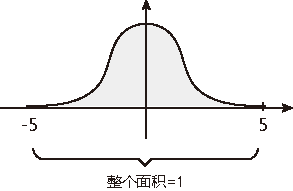
\includegraphics[width=0.45\textwidth]{/0192.pdf}  \\

即: \\
\begin{tabular}{|l|l|l|}
	\hline
	标准正态分布 & 概率函数 $\varphi _0(x)$  & 累加函数 $\Phi _0(x)$ \\
	\hline
	当 $x \leq -5$ 时 & $y \approx 0$ & $y \approx 0$\\
	\hline
	当 $x \geq 5$ 时 & $y \approx 0$ & $y \approx 1$\\
	\hline
\end{tabular} \\








\section{普通的``正态分布", 怎样转化成``标准正态分布"?}

\subsection{``概率函数"的转化公式是: $\boxed{
	\varphi (x)=\frac{1}{\sigma}\cdot \varphi _0(\frac{x-\mu}{\sigma})
	}$}

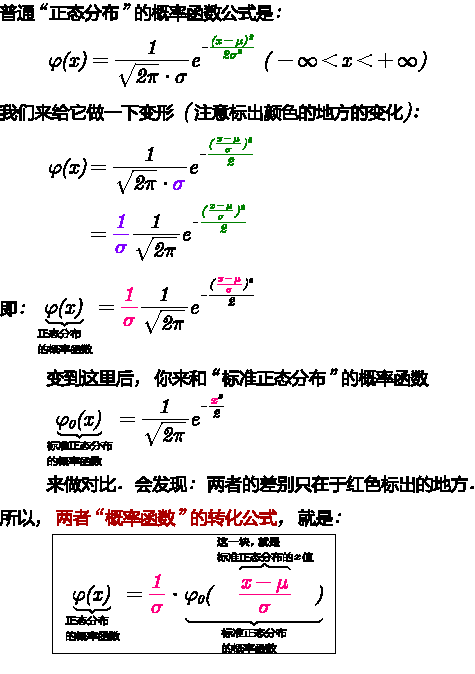
\includegraphics[width=0.6\textwidth]{/0193.pdf} \\




\begin{myEnvSample}
	你每天等公交的时间, 是一个随机变量X,这个变量服从正态分布. 过去20天, 你等公交的时间(分钟)分别是: 26,33,65,28,34,55,25,44,50,36,26,37,43,62,35,38,45,32,28,34. \\
	那么, 你现在等公交会耗费30-45分钟的概率是多少? --- 即求:  P(30 < X < 45). \\
	
	
	\underline{第1步: 先算``正态分布":所需要的两个参数: 均数$\mu$, 标准差$\sigma$.} \\
	- 均数$\mu$ = 38.8 (分钟) \\
	- 标准差$\sigma$ = 11.4 (分钟) \\


	\underline{第2步: 把``正态分布", 转成``标准正态分布"(即做``z变换")} \\
	转换后,  ``正态分布"中的$\mu=38.8, \ \sigma=11.4$, 就能变成``标准正态分布"中的$\mu=0, \ \sigma=1$. \\
	
	``标准化(z变换)"的转换公式是: $\boxed{
		new X= \frac{oldX- \mu} {\sigma} 
	}$ \\
	原始的``正态分布"是 P(30 < X < 45). \\
	我们把 30 和 45, 分布代入上面转换公式中: \\
	- 对于30, z变换后的值, 就是: $newX=\frac{oldX-\text{均值}\mu}{\text{标准差}\sigma}=\frac{30-38.8}{11.4}=-0.77193	$ \\
	- 对于40, z变换后的值, 就是: $newX=\frac{oldX-\text{均值}\mu}{\text{标准差}\sigma}=\frac{45-38.8}{11.4}=0.54386	$ \\
	
	这样后, 原始的 $P(30 \leq X \leq 45)$ 就被我们转换成了:  $P(-0.77 \leq Z \leq 0.54)$ \\
	
	\textbf{经过``标准化"转换后,原来的正态曲线的形状不会变化,即不会改变胖瘦,只是位置发生平移.} \\
	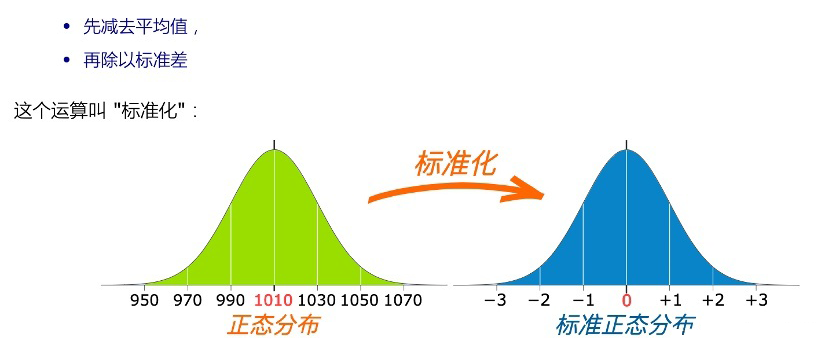
\includegraphics[width=0.95\textwidth]{/0210.png} \\ 


	\underline{第3步: 完成z变换后,我们能利用``z值表", 来找到对应的概率值.} \\
	
	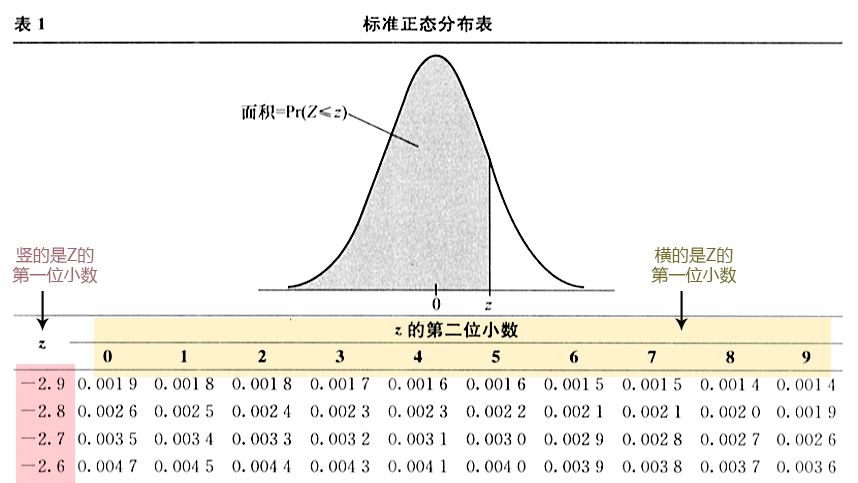
\includegraphics[width=1\textwidth]{/0211.png} \\	
	注意: \textbf{图中阴影部分的面积, 代表的是: $Z \leq z$的概率.} (注意是``$\leq$"). \\	
	
	所以, 本例要求的 $P(-0.77 \leq Z \leq 0.54)$, 就等于 $= P(Z \leq 0.54) – P(Z \leq -0.77)$ \\
	因此, 我们只要找到 $Z \leq 0.54$ 和 $Z \leq -0.77$ 对应的概率值后, 直接把它们相减, 就能得到答案. \\
	
	- 先看 $Z \leq 0.54$ 的P值.  第一个小数是5, 就在表格的最左边那一列,找到0.5. 第二个小数是4,就定位到``顶行"的4那一列. 得到 0.7054. \\
	- 同理, 找到 $Z \leq -0.77$ 对应的P值, 是0.2206. \\
	
	所以,
	\begin{align*}  % 支持每行编号. 若不需要编号, 就用 align*环境
P\left( -0.77\leq Z\leq 0.54 \right) &=P\left( Z\leq 0.54 \right) –P\left( Z\leq -0.77 \right) \\
&=0.7054-0.2206=0.4848
	\end{align*}

所以, 你现在等公交会耗费30-45分钟的概率, 会达到48\%. \\
	
	其实, 在geogebra中可以直接用``正态分布"的均值和标准差来做, 不需要转换成``标准正态分布". \\
	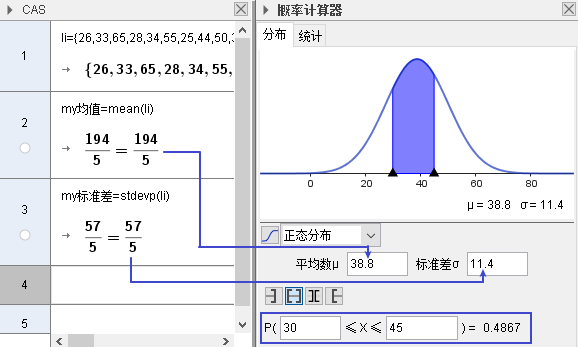
\includegraphics[width=0.95\textwidth]{/0209.png} 	
	
\end{myEnvSample}




\subsection{``累加函数"的转化公式是: $\boxed{\varPhi (x)=\varPhi _0(\frac{x-\mu}{\sigma})	}$}

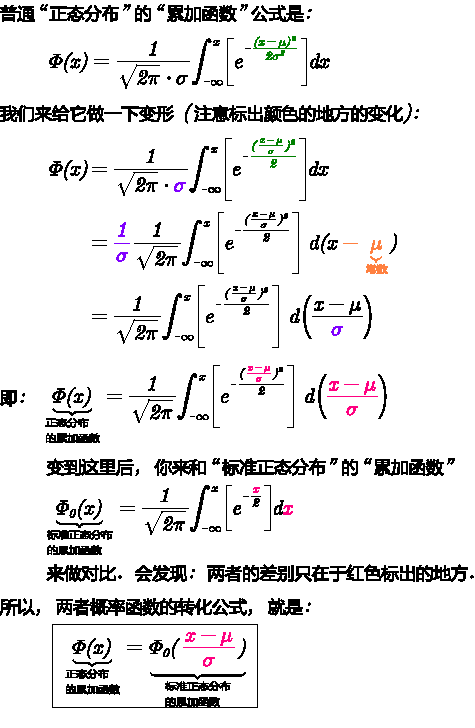
\includegraphics[width=0.6\textwidth]{/0194.pdf} \\




\begin{myEnvSample}
有 $X \sim N(1,4)$, 即 $\mu=1, \ \sigma^2=4,\ \sigma=2$ \\
到注意: 这只是一个普通的正态分布, 我们必须先把它转成``标准正态分布"再来做. \\

→ 求 $P\{0<X<1.6\} =\varPhi (1.6)-\varPhi (0)$ \\
先把这个累加函数$\Phi (x)$ (正态分布的), 转成$\Phi_0 (x)$ (标准正态分布的). 套用转化公式, 就有: \\
$	\varPhi (1.6)=\varPhi _0\left( \frac{x-\mu}{\sigma} \right) =\varPhi _0\left( \frac{1.6-1}{2} \right) =\varPhi _0(0.3)$ \\
$	\varPhi (0)=\varPhi _0\left( \frac{x-\mu}{\sigma} \right) =\varPhi _0\left( \frac{0-1}{2} \right) =\varPhi _0(-0.5)$ \\

所以回到原题, $
\varPhi (1.6)-\varPhi (0)=\varPhi _0(0.3)-\underset{=1-\varPhi _0(0.5)}{\underbrace{\varPhi _0(-0.5)}}
$ \\

→ 求 $P\left\{ |X|\leq 2 \right\} $ \\
方法1: 
\begin{align*}  % 支持每行编号. 若不需要编号, 就用 align*环境
	P\left\{ |X|\leq 2 \right\} &=P\left\{ -2\leq X\leq 2 \right\}\\
&=\varPhi \left( 2 \right) -\varPhi \left( -2 \right) \ \gets \text{转成} \text{``标准正态分布"}”\text{的累加函数}\\
&=\varPhi _0\left( \frac{2-\overset{\mu}{\overbrace{1}}}{\underset{\sigma}{\underbrace{1}}} \right) -\varPhi _0\left( \frac{-2-1}{1} \right)\\
&=\varPhi _0\left( 0.5 \right) -\varPhi _0\left( -1.5 \right)\\
&=\varPhi _0\left( 0.5 \right) -\left[ 1-\varPhi _0\left( 1.5 \right) \right]
\end{align*} 

方法2: 
\begin{align*}  % 支持每行编号. 若不需要编号, 就用 align*环境
	P\left\{ |X|\leq 2 \right\}
&=P\left\{ -2\leq X\leq 2 \right\}\\
&=P\left\{ \left( -2-1 \right) \leq \left( X-1 \right) \leq \left( 2-1 \right) \right\} \ \gets \text{对}X\text{左中右,同时减去}\mu \text{值}1\\
&=P\left\{ \frac{-2-1}{2}\leq \frac{X-\overset{\mu}{\overbrace{1}}}{\underset{\sigma}{\underbrace{2}}}\leq \frac{2-1}{2} \right\} \ \gets \text{对}X\text{左中右,同时除以}\sigma \text{值}2\\
&\text{注意,现在中间的}\frac{X-1}{2},\text{就已经被我们转化成了``标准正态分布"的x形式了},\\
&\text{即从}x\text{转成了}\frac{x-\mu}{\sigma}\\
&=P\left\{ -1.5\leq \frac{X-1}{2}\leq 0.5 \right\}\\
&=\varPhi _0\left( 0.5 \right) -\varPhi _0\left( -1.5 \right)
\end{align*}

\end{myEnvSample}
\vspace{1em} 




\begin{myEnvSample}
飞船零件, 尺寸符合``正态分布" $X\sim N\left( \underset{\mu}{\underbrace{50}},\underset{\sigma ^2}{\underbrace{1}} \right) $, 即 $\sigma=1$ \\
其尺寸只有在 $50 \pm 1$ 时, 才是合格的. \\

那么问:  \\
→ 生产出的单个飞船零件, 合格概率是? 
\begin{align*}  % 支持每行编号. 若不需要编号, 就用 align*环境
	P\left\{ 49\leq X\leq 51 \right\} 
&=\varPhi \left( 51 \right) -\varPhi \left( 49 \right)\\
&=\varPhi _0\left( \frac{51-\overset{\mu}{\overbrace{50}}}{\underset{\sigma}{\underbrace{1}}} \right) -\varPhi _0\left( \frac{49-50}{1} \right)\\
&=\varPhi _0\left( 1 \right) -\varPhi _0\left( -1 \right)\\
&=\varPhi _0\left( 1 \right) -\left( 1-\varPhi _0\left( 1 \right) \right) =0.68269 
\end{align*}

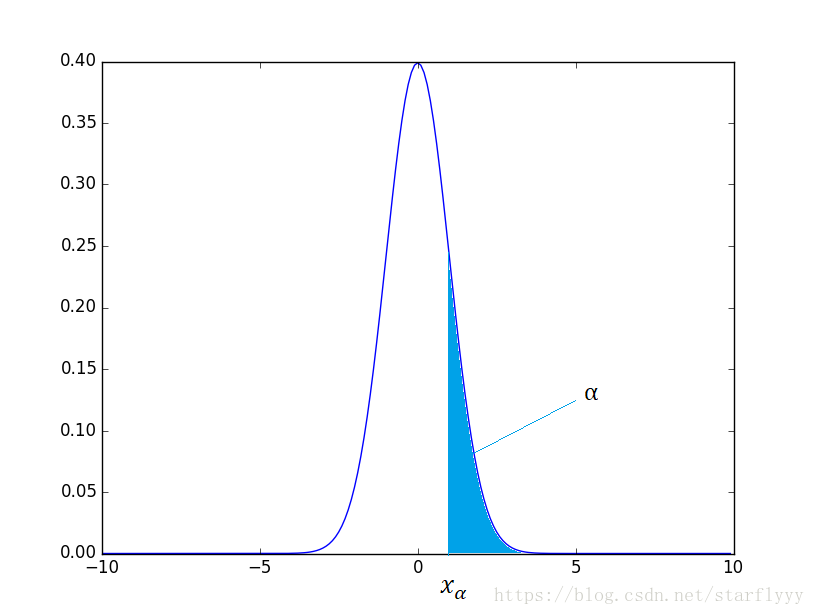
\includegraphics[width=0.5\textwidth]{/0195.png} \\



→ 重复抽检3次, 至少有1个零件是合格的概率?
\begin{align*}  % 支持每行编号. 若不需要编号, 就用 align*环境
	P\underset{\text{我们令}Y\text{表示合格品的数量}}{\underbrace{\left\{ Y\ge 1 \right\} }}
	&=1-\underset{\text{所抽的3件都不合格\ 的概率}}{\underbrace{P\left\{ Y=0 \right\} }}\\
&=1-\left( 1-\underset{\text{单个产品的合格率}}{\underbrace{0.6827}} \right) ^3=0.968054
\end{align*}
\end{myEnvSample}
\vspace{1em} 




\begin{myEnvSample}
X是服从正态分布的, 即 $X\sim N\left( \mu ,\sigma ^2 \right) $, 求: \\
→ 
\begin{align*}  % 支持每行编号. 若不需要编号, 就用 align*环境
	P\{|X-\mu |<\sigma \}
&=P\{-\sigma <X-\mu <\sigma \}\\
&=P\{-\sigma +\mu <X<\sigma +\mu \}\\
&=\varPhi \underset{}{\underbrace{\left( \sigma +\mu \right) }}-\varPhi \underset{}{\underbrace{\left( -\sigma +\mu \right) }}\ \gets \text{先转成``标准正态分布"的}\varPhi _0\\
&=\varPhi _0\left( \frac{\overset{}{\overbrace{(\sigma +\mu )}}-\mu}{\sigma} \right) -\varPhi _0\left( \frac{\overset{}{\overbrace{(-\sigma +\mu )}}-\mu}{\sigma} \right)\\
&=\varPhi _0(1)-\varPhi _0(-1)\\
&=\varPhi _0(1)-\left[ 1-\varPhi _0(1) \right] =0.6827 
\end{align*}

→ $P\{|X-\mu |<2\sigma \} = ?$ 根据上面的方法, 同理= 0.9544 \\
→ $P\{|X-\mu |<3\sigma \} = ?$ 根据上面的方法, 同理= 0.9974 \\

这个例题, 就引出了 ``3σ准则".
\end{myEnvSample}



~\\
\hrule
~\\



\section{$3\sigma$ 准则 (pauta criterion)}

对于``标准正态分布 standard normal distribution", 它的均数$\mu=0$,标准差$\sigma =1$. \\
因为标准差$\sigma =1$. 所以在x轴上: \\
- 1倍的$\sigma$, 就=1;  \\
- 两倍的$\sigma$, 就=2; \\
- 三倍的$\sigma$, 就=3. \\

并有: \\
- 68\%的数值, 是在离``平均值$\mu$" 1个标准差$\sigma$之内. \\
- 95\%的数值, 是在离``平均值$\mu$" 2个标准差$\sigma$之内. \\
- 99.7\%的数值, 是在离``平均值$\mu$" 3个标准差$\sigma$之内. \\
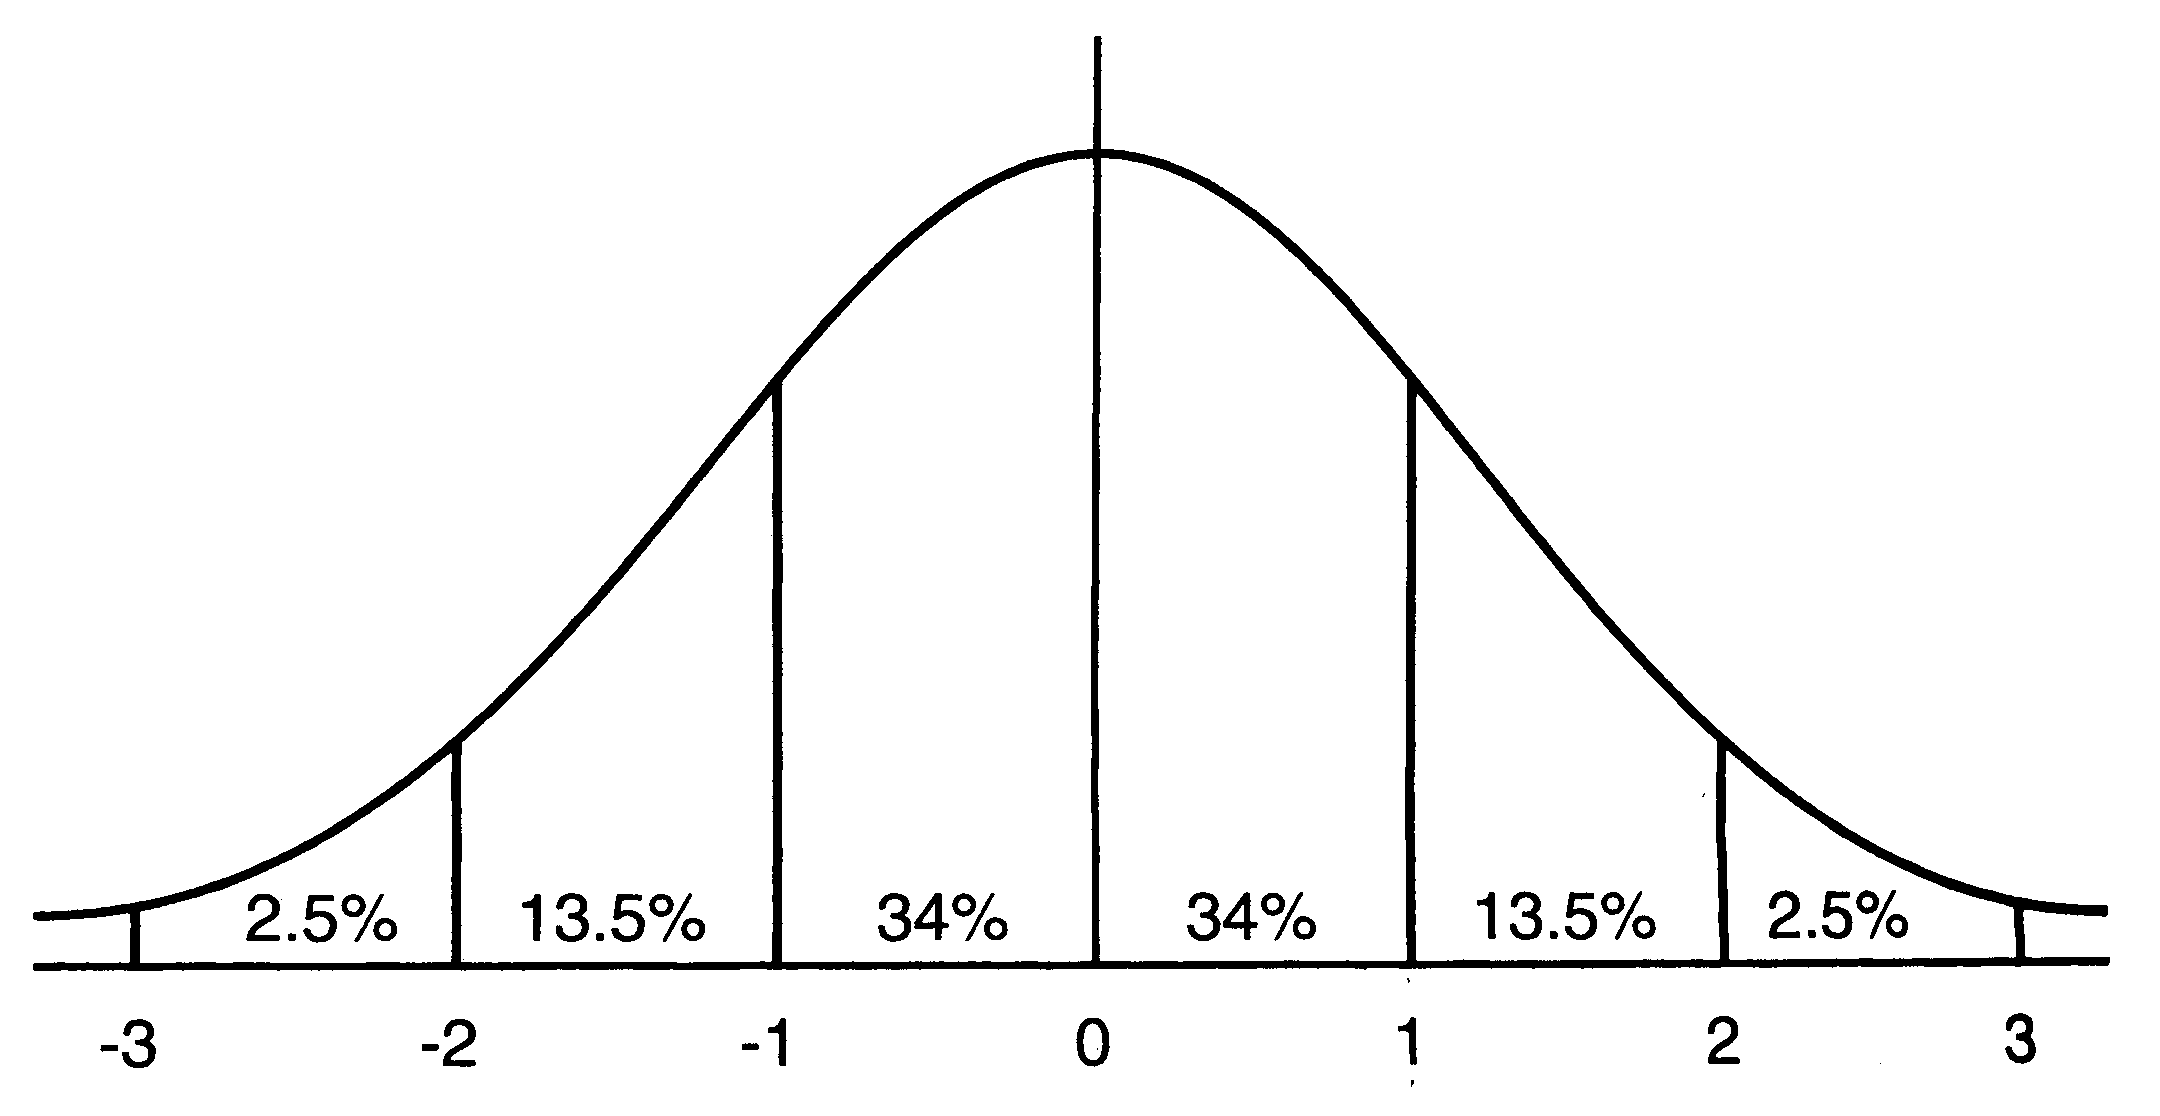
\includegraphics[width=0.55\textwidth]{/0213.png} \\

也就是说, 在[-1,1]这个区间就包含了它可以取的68\%的值,[-2,2]区间包含了95\%的值,[-3,3]包含了它可能取的99.7\%的值. 这里的1,2,3分别代表一个、两个, 和三个标准差. \\

落在$|3\sigma|$ 区间段内的概率, 是0.99 \\
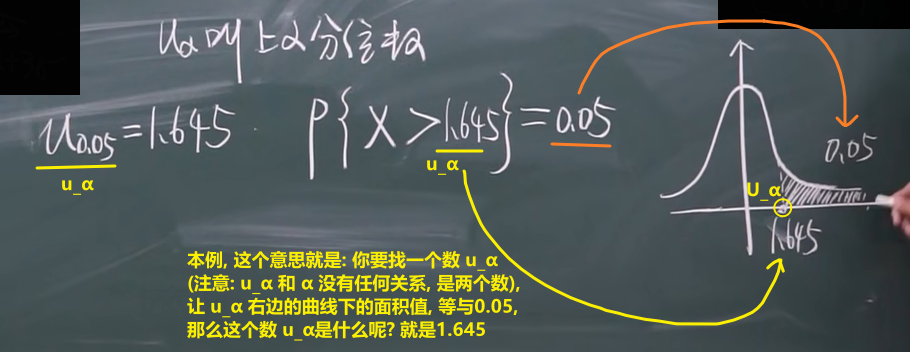
\includegraphics[width=0.55\textwidth]{/0196.png}  \\

所以,根据这些统计规律,我们就可以推断出: 一个服从``标准正态分布"的变量,它的取值不太可能超过2,极不可能超过3. (\textbf{因为若它落在$x \geq 3 \sigma = 3$之外, 其概率, 只有 1-99.74\%=0.26\%, 这个概率太小了. 所以这个数值, 极高概率是不属于``标准正态分布"的世界领域中的. 应该被踢出去. 它属于其他的分布世界.}) \\



\begin{myEnvSample}
一些软件, 告诉你开机时间多少秒, 打败了全国97\%的用户, 这个是怎么算出来的? 就是利用了``正态分布模型". \\
只要随机抽取一部分用户的开机数据,算出``均值 $\mu$"和``标准差 $σ$",就可以确定一条正态分布曲线. 在正态分布中,一个标准差, 覆盖68.26\%的数据; 两个标准差, 覆盖95.44\%的数据. 软件\textbf{只需要比较你的``开机时间"离``均值 $\mu$"的差距,就能知道你距离均值多少个标准差 $σ$,也就知道你的排名了.} \\

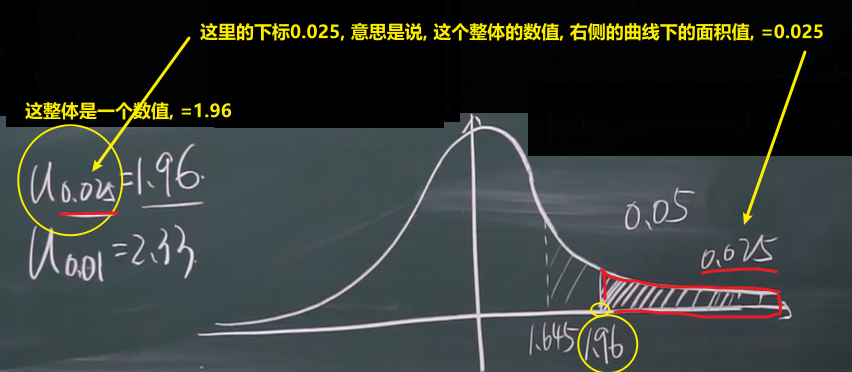
\includegraphics[width=0.6\textwidth]{/0197.png}  
\end{myEnvSample}

所以, 正态分布,为我们提供了一个``估算个体在整体中位置"的便捷方法. 像智商、身高、考试成绩,只要服从``正态分布", 都能使用这种方法, 快速得到答案. \\


\begin{myEnvSample}
	某小学, 学生身高的数据有: \\
	- 平均值$\mu$ = 1.4米 \\
	- 标准差$\sigma$ = 0.15米 \\
	
	人的身高服从``正态分布"的. 我们就可以知道: \\
	- \textbf{这个学校有68\%的学生, 身高会在1.25到1.55米之间. 这首尾两个数值, 就是 ``均值1.4" 加减 ``标准差0.15" 得到的 (均数加减一个标准差).} \\
	- 有95\%的学生, 身高在1.1到1.7之间("均数"加减两个"标准差"得到) \\
	
	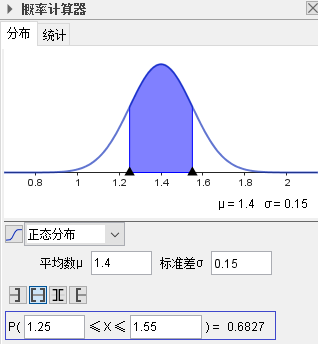
\includegraphics[width=0.55\textwidth]{/0214.png} \\
	
	
	反过来计算也行, 如果我们知道了某个变量的``标准正态分布"的``95\%区间的取值", 我们就可以算出对应的``均数"和``标准差",进而就能知道一切. \\
	
	例如, 学校里, 有95\%的学生, 身高在1.1-1.7m 之间. 则: \\
	- 其均值$\mu$ = (1.1m+1.7m)/2 =1.4m \\
	- 既然 95\%的数据, 击中在 x轴上的 1.1-1.7之间, 而95\%, 是$\mu \pm 2\sigma$ 的横跨幅度(即4个$\sigma$), 所以即: $1.7m-1.1m=0.6m=4\sigma $ \\
	从而得到 1个 $\sigma =\frac{0.6m}{4}=0.15m	$ \\
	
	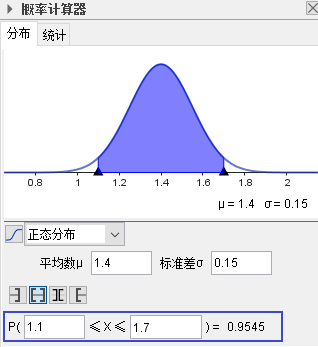
\includegraphics[width=0.55\textwidth]{/0215.png} 
\end{myEnvSample}





\end{document}